\subsection{Scenario Pianificazioni}
\begin{figure}[H] 
    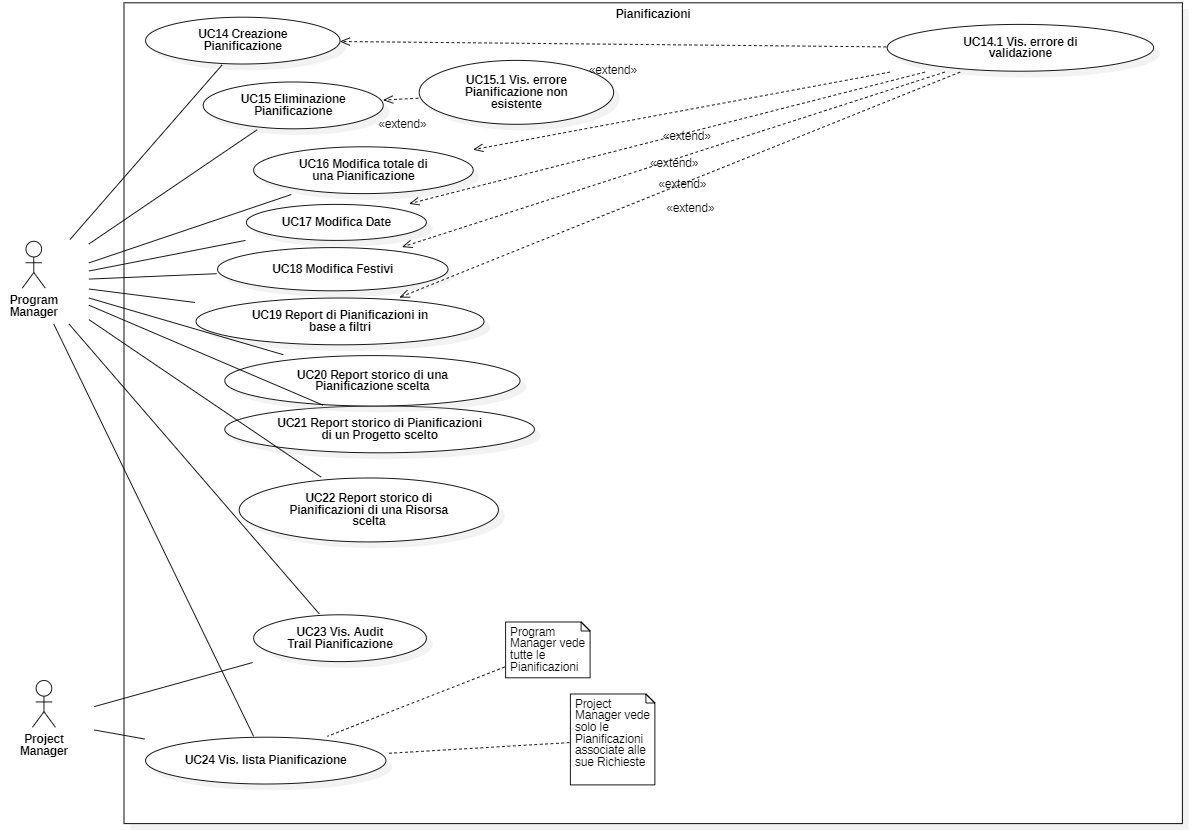
\includegraphics[width=1.00\linewidth]{usecase/pianificazioni-general} 
    \caption{Casi d'Uso del scenario Pianificazioni}
\end{figure}

\subsubsection*{UC16 - Creazione Pianificazione}
\begin{itemize}[label=$\circ$]
\item \textbf{Attore:} Program Manager;
\item \textbf{Descrizione:} il Program Manager può creare una Pianificazione per Figura richiesta da una Richiesta;
\item \textbf{Precondizioni:} il richiedente è un Program Manager;
\item \textbf{Postcondizioni:} la Pianificazione è stata creata dal Program Manager con successo;
\item \textbf{Estensioni:} UC17;
\item \textbf{Inclusioni:} il caso d'uso non ha inclusioni.
\end{itemize}

\subsubsection*{UC17 - Vis. errore di validazione Pianificazioni}
\begin{itemize}[label=$\circ$]
\item \textbf{Attore:} Project Manager e Program Manager;
\item \textbf{Descrizione:} questo caso d'uso descrive anche UC26.2. Viene visualizzato un messaggio di errore in caso vengano eseguite funzionalità con dati non validi. Esso rappresenta i seguenti errori comuni all'interno delle Pianificazioni: dati non validi, filtri non valorizzati, entità associate non valide, risultati nulli o non valorizzati;
\item \textbf{Precondizioni:} il Program Manager o il Project Manager stanno effettuando operazioni con dati non validi;
\item \textbf{Postcondizioni:} l'esecuzione della funzionalità è interrotta e viene visualizzato il messaggio di errore;
\item \textbf{Estensioni:} il caso d'uso non ha estensioni;
\item \textbf{Inclusioni:} il caso d'uso non ha inclusioni.
\end{itemize}

\subsubsection*{UC18 - Eliminazione Pianificazione}
\begin{itemize}[label=$\circ$]
\item \textbf{Attore:} Program Manager;
\item \textbf{Descrizione:} il Program Manager può eliminare una Pianificazione esistente;
\item \textbf{Precondizioni:} il richiedente è il Program Manager;
\item \textbf{Postcondizioni:} la Pianificazione è stata eliminata dal Program Manager con successo;
\item \textbf{Estensioni:} UC17;
\item \textbf{Inclusioni:} il caso d'uso non ha inclusioni.
\end{itemize}

\subsubsection*{UC19 - Modifica Pianificazione}
\begin{itemize}[label=$\circ$]
\item \textbf{Attore:} Program Manager;
\item \textbf{Descrizione:} il Program Manager può modificare una Pianificazione esistente nella sua totalità sovrascrivendola;
\item \textbf{Precondizioni:} il richiedente è un Program Manager;
\item \textbf{Postcondizioni:} la Pianificazione selezionata è stata modificata con successo;
\item \textbf{Estensioni:} UC17;
\item \textbf{Inclusioni:} il caso d'uso non ha inclusioni.
\end{itemize}

\subsubsection*{UC20 - Modifica Date}
\begin{itemize}[label=$\circ$]
\item \textbf{Attore:} Program Manager;
\item \textbf{Descrizione:} il Program Manager può modificare le date di inizio e/o di fine di una Pianificazione;
\item \textbf{Precondizioni:} il richiedente è un Program Manager;
\item \textbf{Postcondizioni:} la Pianificazione è stata modificata con successo solo nel campo Data inizio e/o Data fine dal Program Manager;
\item \textbf{Estensioni:} UC17;
\item \textbf{Inclusioni:} il caso d'uso non ha inclusioni.
\end{itemize}

\subsubsection*{UC21 - Modifica Festivi}
\begin{itemize}[label=$\circ$]
\item \textbf{Attore:} Program Manager;
\item \textbf{Descrizione:} il Porgram Manager può modificare il campo Festivi di una Pianificazione. Se posto a vero il lavoratore potrà lavorare anche nei giorni festivi;
\item \textbf{Precondizioni:} il richiedente è un Program Manager;
\item \textbf{Postcondizioni:}  la Pianificazione è stata modificata con successo solo nel campo Festivi dal Program Manager;
\item \textbf{Estensioni:} UC17;
\item \textbf{Inclusioni:} il caso d'uso non ha inclusioni.
\end{itemize}

\subsubsection*{UC22 - Esportazione file Excel di Pianificazioni in base a filtri}
\begin{itemize}[label=$\circ$]
\item \textbf{Attore:} Program Manager;
\item \textbf{Descrizione:} : il Program Manager può esportare in un
file Excel scaricabile un report delle Pianificazioni in base a dei filtri inseriti;
\item \textbf{Precondizioni:} : il richiedente è un Program Manager;
\item \textbf{Postcondizioni:} il report Excel è stato generato correttamente ed è possibile
scaricarlo;
\item \textbf{Estensioni:} UC17;
\item \textbf{Inclusioni:} il caso d'uso non ha inclusioni.
\end{itemize}

\subsubsection*{UC23 - Esportazione storico Excel di Pianificazioni di un Progetto}
\begin{itemize}[label=$\circ$]
\item \textbf{Attore:} Program Manager;
\item \textbf{Descrizione:} il Program Manager può esportare in un file Excel scaricabile uno storico di Pianificazioni associate ad un Progetto contenente tutte le risorse allocate e l’effettivo impiego di queste nelle attività;
\item \textbf{Precondizioni:} il richiedente è un Program Manager;
\item \textbf{Postcondizioni:} il report Excel è stato generato correttamente ed è possibile
scaricarlo;
\item \textbf{Estensioni:} UC17;
\item \textbf{Inclusioni:} il caso d'uso non ha inclusioni.
\end{itemize}

\subsubsection*{UC24 - Esportazione storico Excel di Pianificazioni di una Risorsa}
\begin{itemize}[label=$\circ$]
\item \textbf{Attore:} Program Manager;
\item \textbf{Descrizione:} il Program Manager può esportare in un file Excel scaricabile uno storico di Pianificazioni in cui c'è stata una determinata Risorsa;
\item \textbf{Precondizioni:} il richiedente è un Program Manager;
\item \textbf{Postcondizioni:} il report Excel è stato generato correttamente ed è possibile
scaricarlo;
\item \textbf{Estensioni:} UC17;
\item \textbf{Inclusioni:} il caso d'uso non ha inclusioni.
\end{itemize}

\subsubsection*{UC25 - Vis. Audit Trail Pianificazione}
\begin{figure}[H] 
    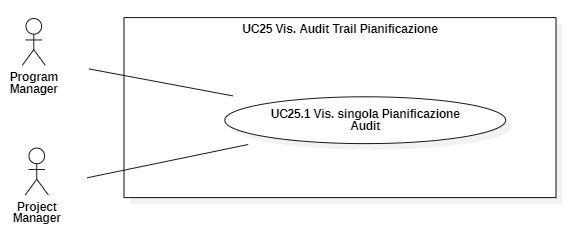
\includegraphics[width=0.65\linewidth]{usecase/UC25} 
    \caption{Caso d'Uso 25 espanso}
\end{figure}

\begin{itemize}[label=$\circ$]
\item \textbf{Attore:} Project Manager o Program Manager;
\item \textbf{Descrizione:} il Project Manager o il Program Manager possono visualizzare
l’audit trail di una Richiesta selezionata. Il Project Manager può vedere solo le tracce di audit delle Pianificazioni associate alle sue Richieste, mentre il Program Manager può vederle tutte;
\item \textbf{Precondizioni:} il richiedente è un Program Manager o un Project Manager;
\item \textbf{Postcondizioni:} la traccia di audit della Pianificazione selezionata è visualizzabile dal Project Manager o dal Program Manager;
\item \textbf{Estensioni:} UC17;
\item \textbf{Inclusioni:} il caso d'uso non ha inclusioni.
\end{itemize}


\subsubsection*{UC25.1 - Vis. singola Pianificazione Audit}
\begin{figure}[H] 
    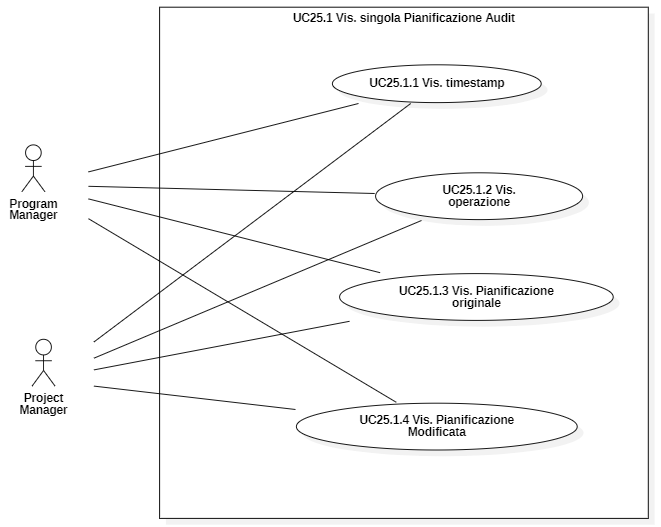
\includegraphics[width=0.75\linewidth]{usecase/UC25.1} 
    \caption{Caso d'Uso 25.1 espanso}
\end{figure}

\begin{itemize}[label=$\circ$]
\item \textbf{Attore:} Project Manager o Program Manager;
\item \textbf{Descrizione:} il Project Manager o il Program Manager può vedere l'audit di una singola Pianificazione. Il Project Manager può vedere solo le Pianificazioni associate alle sue Richieste, mentre il Program Manager può vederle tutte;
\item \textbf{Precondizioni:} l'audit trail è visualizzabile;
\item \textbf{Postcondizioni:} l'audit di una singola Pianificazione è visualizzabile;
\item \textbf{Estensioni:} il caso d'uso non ha estensioni;
\item \textbf{Inclusioni:} il caso d'uso non ha inclusioni.
\end{itemize}

\subsubsection*{UC25.1.1 - Vis. timestamp}

\begin{itemize}[label=$\circ$]
\item \textbf{Attore:} Project Manager o Program Manager;
\item \textbf{Descrizione:} il Project Manager e il Program Manager possono visualizzare il
timestamp di una singola audit di una Pianificazione;
\item \textbf{Precondizioni:} la singola audit di una Pianificazione è visualizzabile;
\item \textbf{Postcondizioni:} il timestamp della singola audit è visualizzabile;
\item \textbf{Estensioni:} il caso d'uso non ha estensioni;
\item \textbf{Inclusioni:} il caso d'uso non ha inclusioni.
\end{itemize}

\subsubsection*{UC25.1.2 - Vis. operazione}

\begin{itemize}[label=$\circ$]
\item \textbf{Attore:} Project Manager o Program Manager;
\item \textbf{Descrizione:} il Project Manager e il Program Manager possono visualizzare l'operazione di una singola audit di una Pianificazione;
\item \textbf{Precondizioni:} la singola audit di una Pianificazione è visualizzabile;
\item \textbf{Postcondizioni:} l’operazione della singola audit è visualizzabile;
\item \textbf{Estensioni:} il caso d'uso non ha estensioni;
\item \textbf{Inclusioni:} il caso d'uso non ha inclusioni.
\end{itemize}

\subsubsection*{UC25.1.3 - Vis. Pianificazione originale}

\begin{itemize}[label=$\circ$]
\item \textbf{Attore:} Project Manager o Program Manager;
\item \textbf{Descrizione:} il Project Manager o il Program Manager possono visualizzare la
singola audit di una Pianificazione prima che l’operazione venga eseguita;
\item \textbf{Precondizioni:}la singola audit di una Pianificazione è visualizzabile;
\item \textbf{Postcondizioni:} la Richiesta originale della singola audit è visualizzabile;
\item \textbf{Estensioni:} il caso d'uso non ha estensioni;
\item \textbf{Inclusioni:} il caso d'uso non ha inclusioni.
\end{itemize}

\subsubsection*{UC25.1.4 - Vis. Pianificazione modificata}

\begin{itemize}[label=$\circ$]
\item \textbf{Attore:} Project Manager o Program Manager;
\item \textbf{Descrizione:} il Project Manager o il Program Manager possono visualizzare la
singola audit di una Pianificazione dopo che l’operazione è stata eseguita;
\item \textbf{Precondizioni:} la singola audit di una Pianificazione è visualizzabile;
\item \textbf{Postcondizioni:} la Pianificazione modificata della singola audit è visualizzabile;
\item \textbf{Estensioni:} il caso d'uso non ha estensioni;
\item \textbf{Inclusioni:} il caso d'uso non ha inclusioni.
\end{itemize}

\subsubsection*{UC26 - Vis. lista Pianificazione}
\begin{figure}[H] 
    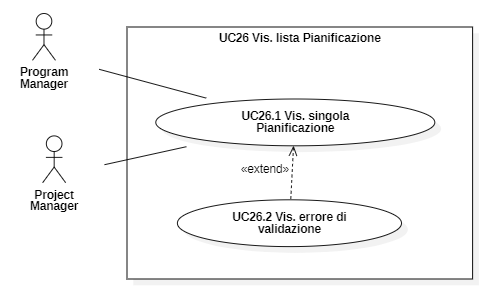
\includegraphics[width=0.65\linewidth]{usecase/UC26} 
    \caption{Caso d'Uso 26 espanso}
\end{figure}

\begin{itemize}[label=$\circ$]
\item \textbf{Attore:}  Project Manager o Program Manager;
\item \textbf{Descrizione:} il Project Manager o il Program Manager possono visualizzare
una lista di Richieste dopo aver inserito filtri e/o una parola nella ricerca rapida
e aver selezionato se i filtri applicati devono essere congiunti o disgiunti. Il Project Manager può vedere solo le Pianificazioni associate alle sue Richieste, mentre il Program Manager può vederle tutte;
\item \textbf{Precondizioni:} il richiedente è un Project Manager o un Program Manager;
\item \textbf{Postcondizioni:} la lista delle Richieste è visualizzabile dal Project Manager o dal Program Manager;
\item \textbf{Estensioni:} UC17;
\item \textbf{Inclusioni:} il caso d'uso non ha inclusioni.
\end{itemize}


\subsubsection*{UC26.1 - Vis. singola Pianificazione}
\begin{figure}[H] 
    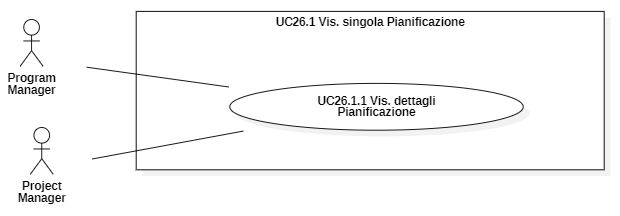
\includegraphics[width=0.75\linewidth]{usecase/UC26.1} 
    \caption{Caso d'Uso 26.1 espanso}
\end{figure}

\begin{itemize}[label=$\circ$]
\item \textbf{Attore:}  Project Manager o Program Manager;
\item \textbf{Descrizione:} il Project Manager o il Program Manager possono visualizzare la Pianificazione selezionata. Il Project Manager può vedere solo le Pianificazioni associate alle sue Richieste, mentre il Program Manager può vederle tutte;
\item \textbf{Precondizioni:} la lista delle Pianificazioni è visualizzabile;
\item \textbf{Postcondizioni:} la Pianificazione selezionata è visualizzabile dal Program Manager o dal Project Manager;
\item \textbf{Estensioni:} UC26.2;
\item \textbf{Inclusioni:} il caso d'uso non ha inclusioni.
\end{itemize}

\subsubsection*{UC26.1.1 - Vis. dettagli Pianificazione}
\begin{itemize}[label=$\circ$]
\item \textbf{Attore:}  Project Manager o Program Manager;
\item \textbf{Descrizione:} il Project Manager o il Program Manager possono visualizzare la
Pianificazione selezionata;
\item \textbf{Precondizioni:} la Pianificazione singola è visualizzabile;
\item \textbf{Postcondizioni:} il Project Manager e il Program Manager possono visualizzare
i campi di una Pianificazione selezionata;
\item \textbf{Estensioni:} il caso d'uso non ha estensioni;
\item \textbf{Inclusioni:} il caso d'uso non ha inclusioni.
\end{itemize}


